\chapter[Search for the deacy $\Bp\!\to\Dsp\phi$]{Search for the deacy $\boldsymbol{\Bp\!\to\Dsp\phi}$}
\label{ch:dsphi}

%So, a lot of this comes from the ANA and PAPER.
%
%
%\begin{figure}
  %\begin{center}
    %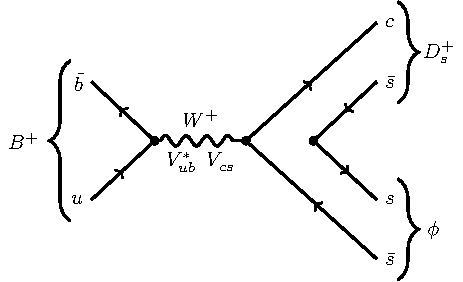
\includegraphics[scale=1]{feynman_dsphi_sm}
    %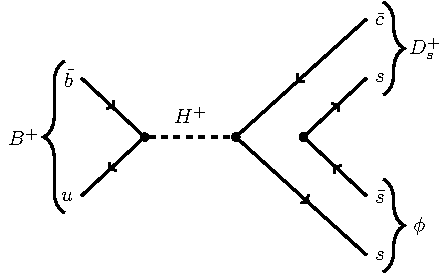
\includegraphics[scale=1]{feynman_dsphi_susy}
  %\end{center}
  %\caption[Feynman diagrams for \btodsphi in SM and BSM]
  %{\small
    %Feynman diagrams
  %}
%\end{figure}
%
%\section{Motivation}
%\begin{itemize}
  %\item First observation, fully hadronic B decay
  %\item CPV in this sector
  %\item Feynmann diagram
%\end{itemize}
%
%
%\section{Theory specific to \btodsphi}
%\begin{itemize}
  %\item CPV again, SUSY
%\end{itemize}
%
%
%\section{Data sample}
%
%
%\section{Selection}
%
%
%\subsection{Multivariate selection --- BDTs}
%\begin{itemize}
  %\item Widely used in (modern) particle physics
  %\item Basic principles
%\end{itemize}
%
%\section{Backgrounds}
%\begin{itemize}
  %\item Combinatorics (define)
  %\item All the specific peaking backgrounds
%\end{itemize}
%
%\section{Results}

